\documentclass[../main]{subfiles}
\begin{document}

\graphicspath{{../figures/}}

\section{検証実験}
本研究では,提案手法の有効性を検証するために,マイクを搭載した台車を移動ロボットに見立て,横2.3m,縦3mの経路を走行させ,異常音源の座標を推定する実験を行った.
正常音のデータは,全てのギアボックスから発せられた正常な運転音を収録したものを用い,異常音のデータは,正常音の収録の際に使用したギアボックスのうち一つに対し
歯車に異物をかませることで発生した音を収録したものを用いた.


正常音のデータと異常音のデータの取得回数はそれぞれ4セットと1セットであり,正常音のデータのうち3セットを学習データ,1セットを検証データとして用いた.
以下に,移動ロボットの経路とギアボックスの音源の配置を示す.


異常音源の正確な座標は,\reffig{route}に示す経路上の座標(0.5, -0.3)とした.
実験に用いたマイクのサンプリング周波数は44.1kHz,前処理に用いた短時間フーリエ変換のウィンドウサイズは65536,スライド幅は1024,メルフィルタバンクの数は128とした.
\begin{figure}[tb]
  \centering
  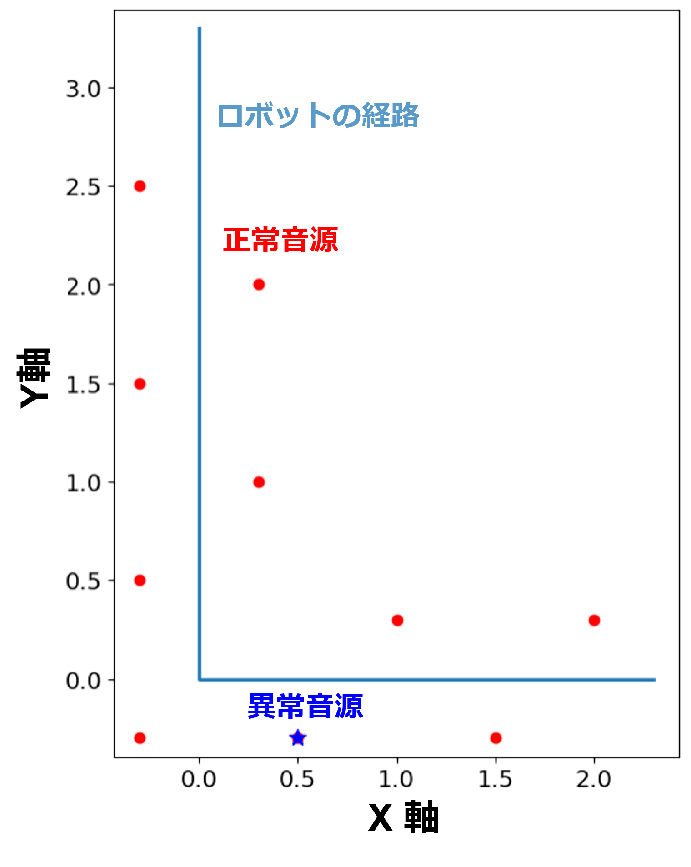
\includegraphics[keepaspectratio, width=0.8\linewidth]{route.pdf}
  \caption{移動ロボットの経路}
  \labfig{route}
\end{figure}

\end{document}
